\documentclass[a4paper,11pt]{article}
		\usepackage[utf8]{inputenc}
	\usepackage[italian]{babel}
	\usepackage{hyperref}	%Consente l'inserimento di \url
	\usepackage{booktabs}	%Utilità di abbellimento tabelle
	\usepackage{longtable}
	\usepackage{tabularx}
	%\usepackage{widetable}
	\usepackage{array}
	\usepackage{listings}
	\usepackage{graphicx}
	\usepackage{caption}
	\usepackage{fancyhdr}
	\newenvironment{fixpic}{}{} % [1]
	\usepackage[a4paper,top=3cm,bottom=3cm,left=2.5cm,right=2.5cm]{geometry}
	%******
	\usepackage{makeidx}
	\usepackage{textcomp}
	\usepackage{multirow}
	\usepackage{rotfloat}
	\usepackage{lastpage}
	\usepackage{array}
	\usepackage{float}
	% *************************************
	% QUI CODICE PER \SUBSUBSUBSECTION
	\usepackage{titlesec}
	\titleclass{\subsubsubsection}{straight}[\subsection]
	
	\newcounter{subsubsubsection}[subsubsection]
	\renewcommand\thesubsubsubsection{\thesubsubsection.\arabic{subsubsubsection}}
	\renewcommand\theparagraph{\thesubsubsubsection.\arabic{paragraph}} % optional; useful if paragraphs are to be numbered
	
	\titleformat{\subsubsubsection}
	  {\normalfont\normalsize\bfseries}{\thesubsubsubsection}{1em}{}
	\titlespacing*{\subsubsubsection}
	{0pt}{3.25ex plus 1ex minus .2ex}{1.5ex plus .2ex}
	
	\makeatletter
	\renewcommand\paragraph{\@startsection{paragraph}{5}{\z@}%
	  {3.25ex \@plus1ex \@minus.2ex}%
	  {-1em}%
	  {\normalfont\normalsize\bfseries}}
	\renewcommand\subparagraph{\@startsection{subparagraph}{6}{\parindent}%
	  {3.25ex \@plus1ex \@minus .2ex}%
	  {-1em}%
	  {\normalfont\normalsize\bfseries}}
	\def\toclevel@subsubsubsection{4}
	\def\toclevel@paragraph{5}
	\def\toclevel@paragraph{6}
	\def\l@subsubsubsection{\@dottedtocline{4}{7em}{4em}}
	\def\l@paragraph{\@dottedtocline{5}{10em}{5em}}
	\def\l@subparagraph{\@dottedtocline{6}{14em}{6em}}
	\makeatother
	
	\setcounter{secnumdepth}{4}
	\setcounter{tocdepth}{4}
	%FINE \SUBSUBSUBSECTION
	%****************************************
	%STYLE PER INSERIMENTO DEL CODICE
	\lstdefinestyle{style1}{
	  belowcaptionskip=1\baselineskip,
	  breaklines=true,
	  frame=L,
	  xleftmargin=\parindent,
	  language=Pascal,
	  showstringspaces=false,
	  basicstyle=\footnotesize\ttfamily,
	  keywordstyle=\bfseries\color{blue},
	  commentstyle=\itshape\color{blue},
	  identifierstyle=\color{blue},
	  stringstyle=\color{orange},
	}
	
	\lstdefinestyle{style2}{
	  belowcaptionskip=1\baselineskip,
	  frame=L,
	  xleftmargin=\parindent,
	  language=C,
	  basicstyle=\footnotesize\ttfamily,
	  commentstyle=\itshape\color{blue},
	}
	\lstset{style=style1}
	
	%FINE STYLE INSERIMENTO CODICE
	%*****************************************
	\usepackage[default]{cantarell} %% Use option "defaultsans" to use cantarell as sans serif only
	\usepackage[T1]{fontenc}        %% for font
	\hypersetup{colorlinks, linkcolor=black, urlcolor=blue}
	\newcommand{\addglos}{\begin{scriptsize}{\textbf{\ped{G}}} \end{scriptsize}} 
	\pagestyle{fancy}
	\fancyhead{}
	\fancyfoot{}
	%\fancyhead[L]{
\includegraphics[scale=0.28]{team_not_found.jpeg}}
	\fancyhead[L]{
\includegraphics[scale=0.15]{../../team404_small.jpg} \hspace{2mm} QUIZZIPEDIA}
	\fancyhead[R]{\leftmark}
	\fancyfoot[L]{Universit\`a degli studi di Padova - IS 2015/2016 \\ \url{team404swe@gmail.com}}

	
	%Commando usato per la tabella di informazioni sul documento
	\newcommand{\introtab}[9]{
		\begin{table}[ht]
		\begin{center}		
		\begin{tabular}{r l}			
			\toprule		
			\multicolumn{2}{c}{\textbf{ Informazioni sul documento }} \\
			\midrule 
			\textbf{Nome Documento}			& \vline \hspace{3.5 mm} {#1} \\
			\textbf{Versione}				& \vline \hspace{3.5 mm} {#2} \\
			\textbf{Uso} 					& \vline \hspace{3.5 mm} {#3} \\
			\textbf{Data Creazione} 		& \vline \hspace{3.5 mm} {#4} \\
			\textbf{Data Ultima Modifica} 	& \vline \hspace{3.5 mm} {#5} \\
			\textbf{Redazione}				& \vline \hspace{3.5 mm} {#6} \\
											%& \vline \hspace{3.5 mm} {#7} \\	
			\textbf{Verifica} 				& \vline \hspace{3.5 mm} {#7}	\\
			\textbf{Approvazione}			& \vline \hspace{3.5 mm} {#8}\\	
			\textbf{Committente} 			& \vline \hspace{3.5 mm} Zucchetti SPA\\
			\textbf{Lista di distribuzione} & \vline \hspace{3.5 mm} Prof. Vardanega Tullio \\														& \vline \hspace{3.5 mm} TEAM404 \\
	\bottomrule	
	\end{tabular}
	\end{center}
	\end{table}
	}
	% Comando di inizio del registro
	\newcommand{\beginregistro}{
		%\begin{longtable}{{|p{0.10\textwidth}|p{0.20\textwidth}|p{0.15\textwidth}|p{0.50\textwidth}|}}
		\begin{longtable}{{|p{1.5cm}|p{2.5cm}|p{2cm}|p{8cm}|}} 
	 		\hline	
	}
	% commando usato pr inserire una riga al registro delle modifiche
	\newcommand{\rigaregistro}[4]{
		{\footnotesize #1} & {\footnotesize #2} &  {\footnotesize #3} &  {\footnotesize #4} \\
			\hline	
	}
	% Comando di fine registro
	\newcommand{\fineregistro}{ \end{longtable}	}
	
	%************************************************
	% commandi per il GLOSSARIO
	%***********************************************
	% Commando di inizio tabella Glossario
	\newcommand{\beginglos}{
		\begin{longtable}{{p{0.20\textwidth}p{0.65\textwidth}}}	
	}
	% Commando per i termini del glossario
	
	\newcommand{\itemglos}[2]{
		\textbf{#1 :} & {#2} \\ \\ \\
	}
	% Commando fine Glossario
	\newcommand{\fineglos}{ \end{longtable} }
	% Comando per aggiungere una ssezione numerata con lettere al glossario
	\newcommand{\sezione}{
	\subsection{}	
	\rule[0.3pt]{\linewidth}{0.4pt} \\ % Linea orizzontale
	}
	
\newcommand{\sezioneglos}[1] { 
  \newpage
  \cleardoublepage
  \phantomsection
  \addcontentsline{toc}{section}{#1}
  \vspace{11pt}
  \textbf{\huge{#1} } % Lettera grande 
  \\
  \rule[0.3pt]{\linewidth}{0.4pt} \\ % Linea orizzontale
  \fancyhead[R]{#1}
}

	\title{\textbf{{\fontsize{8mm}{5mm}\selectfont QUIZZIPEDIA}}}
	\date{}
	\author{}	


\begin{document}
	\maketitle
	\thispagestyle{empty}
	\begin{center}	
	
\includegraphics{../team_not_found.jpg}\\
	\fontsize{5mm}{3mm}\url{team404swe@gmail.com}\\
	
	\vspace{50mm}
	\textbf{Specifica Tecnica 1.0}
	\end{center}
	\introtab{Specifica Tecnica 1.0}			%1 nome documento
			{1.0} 							%2 versione
			{Esterno} 						%3 Uso
			{22 aprile 2016} 				%4 Data cre
			{\today} 						%5 Data mod
			{M. Crivellaro - L. Alessio}	%6 Redazione
			{Alex Beccaro } 			%7 Verifica
			{Martin V. Mbouenda} 				%8 Approvazione
	\newpage
	\thispagestyle{empty}
	\null  

	\newpage
	\newpage
	\fancyhead[R]{REGISTRO DELLE MODIFICHE}
	\fancyfoot[R]{\thepage}
	
	\hspace{30 mm}
	\section*{Registro delle modifiche}
	
	\beginregistro
	
	\rigaregistro{\textbf{Versione}}{\textbf{Autore}}{\textbf{Data}}		 {\hspace{5 mm} 
	\textbf{Descrizione}}
	\rigaregistro{0.1.0}{Luca Alessio (Progettista)}{30/04/2016}{Prima stesura sezioni "Package della componente View" e "Diagrammi delle classi del View"}	
	\rigaregistro{0.0.6}{Davide Bortot (Progettista)}{28/04/2016}{Stesura delle sezioni §2.2, §2.3, §2.4 con la descrizione d'alto livello delle componenti MVP.}
	\rigaregistro{0.0.5}{Luca Alessio (Progettista)}{27/04/2016}{Stesura parziale sezione "Tecnologie e strumenti utilizzati"}
	\rigaregistro{0.0.4}{Davide Bortot (Progettista)}{25/04/2016}{Ampliata la sezione "Architettura generale del sistema".}
	\rigaregistro{0.0.3}{Luca Alessio (Progettista)}{24/04/2016}{Stesura parziale sezione "Architettura generale del sistema"}
	\rigaregistro{0.0.2}{Davide Bortot (Progettista)}{23/04/2016}{Strutturazione iniziale del documento e stesura sezione introduttiva}
	\rigaregistro{0.0.1}{Marco Crivellaro (Progettista)}{22/04/2016}{Creazione documento.}
	\fineregistro

	\newpage
	\fancyhead[R]{\leftmark}
	\tableofcontents
	\pagenumbering{Roman}
	\newpage
	\listoffigures
	\listoftables
	
	\newpage
	\pagenumbering{arabic}
	
	\section*{Sommario}
	
	
	\newpage
	\section{Introduzione}
	\subsection{Scopo del documento}
	
	
	\subsection{Scopo del prodotto}
	Il progetto \textbf{Quizzipedia} ha come obiettivo lo sviluppo di un sistema software basato su tecnologie Web (Javascript\addglos, Node.js\addglos, HTML5\addglos, CSS3\addglos) che permetta la creazione, gestione e fruizione di questionari. Il sistema dovrà quindi poter archiviare i questionari suddivisi per argomento, le cui domande dovranno essere raccolte attraverso uno specifico linguaggio di markup (Quiz Markup Language) d'ora in poi denominato QML\addglos. In un caso d'uso a titolo esemplificativo, un "esaminatore" dovrà poter costruire il proprio questionario scegliendo tra le domande archiviate, ed il questionario così composto sarà presentato e fruibile all' "esaminando", traducendo l'oggetto QML in una pagina HTML\addglos, tramite un'apposita interfaccia web. Il sistema presentato dovrà inoltre poter proporre questionari preconfezionati e valutare le risposte fornite dall'utente finale.
	\\
	Per un'analisi più precisa ed approfondita del progetto si rimanda al documento\\ "\textit{analisi\_dei\_requisiti\_2.0.pdf}".
	\subsection{Glossario}
	Viene allegato un glossario nel file ``\textit{glossario\_2.0.pdf}'' nel quale viene data una definizione a tutti i termini che in questo documento appaiono con il simbolo '\addglos' a pedice.
	\subsection{Riferimenti}
		\subsubsection{Normativi}
		\begin{itemize}
			\item Capitolato d'appalto Quizzipedia:\\
			\url{http://www.math.unipd.it/~tullio/IS-1/2015/Progetto/C5.pdf}
			\item Norme di Progetto: "\textit{norme\_di\_progetto\_2.0.pdf}"
		\end{itemize}
		\subsubsection{Informativi}
		\begin{itemize}
			\item Corso di Ingegneria del Software anno 2015/2016:\\
			\url{http://www.math.unipd.it/~tullio/IS-1/2015/}
			\item Regole del progetto didattico:\\
			\url{http://www.math.unipd.it/~tullio/IS-1/2015/Dispense/PD01.pdf}
			\url{http://www.math.unipd.it/~tullio/IS-1/2015/Progetto/}\\
			\end{itemize}
	\pagebreak
	\newpage
	\section{Specifiche del prodotto}
	I contenuti della specifica saranno presentati seguendo l'approccio top-down: dalla descrizione macroscopica del sistema si scenderà sempre più in dettaglio passando alla descrizione delle singole componenti. Verranno inoltre descritti i design pattern utilizzati e come essi sono stati applicati. Per agevolare la comprensione si è scelto di utilizzare i diagrammi dei package, delle classi, di attività e di sequenza, descritti attraverso lo standard UML 2.0.
	
	\subsection{Architettura generale del sistema}
	Il sistema Quizzipedia è di tipo \emph{client-server}; il \emph{client} fornisce all'utente un'interfaccia web su browser per la creazione e fruizione di questionari, mentre il lato \emph{server} si occupa di gestire e salvare i dati su DBMS PostgreSQL. La base di dati raccoglie principalmente quesiti memorizzati in QML, che su richiesta verranno elaborati da un interprete.
Il suddetto interprete processa l'input QML, precedentemente validato nella forma da un parser apposito, traducendolo in linguaggio HTML5 visualizzabile da browser.
<<<<<<< HEAD
Nella realizzazione del sistema Quizzipedia verrà adottato il design pattern \emph{Model View Presenter} nella sua variante \emph{Passive View}.
\begin{center}
	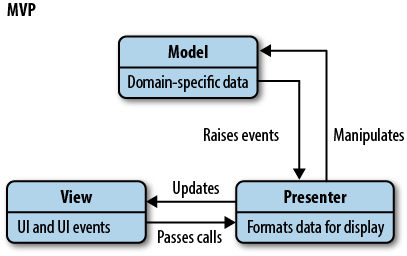
\includegraphics[scale=1.3]{../images/mvp.png}
\end{center}
\begin {itemize}
\item\textbf{Model}: definisce l'organizzazione dei dati e ne specifica le modalità di accesso. Nel sistema Quizzipedia è situato nella parte server che opera sulla sottostante base di dati. Fa parte del Model anche la componente \emph{Parser} che opera sui dati prima che essi vengano salvati nel DBMS.
\item\textbf{View (Passive)}: rappresenta l'interfaccia grafica presentata all'utilizzatore, la quale visualizza i dati e cattura le interazioni dell'utente. L'aggettivo "Passive" indica che la View non è responsabile del proprio aggiornamento al variare del Model, compito che ricade sul Presenter.
\item\textbf{Presenter}: controlla la View e ne gestisce il comportamento in reazione alle interazioni dell'utente, interagisce di conseguenza col Model per ottenere i dati necessari.
Una volta ottenuti i dati si preoccupa di aggiornare la View. Nel sistema Quizzipedia implementa la parte logica, affiancata a quella grafica, del Client. Realizza un totale disaccoppiamento tra Model e View, controllandone i flussi di comunicazione.
	\end {itemize}
	Altre possibili architetture che sono state prese in considerazione sono definite dai design pattern \emph{Model View Controller (MVC)} con \emph{Front Controller}, \emph{Model View Presenter (MVP)} nelle varianti \emph{Presentation Model} e \emph{Supervising Controller}, e il design pattern \emph{Model View ViewModel (MVVM)}.
	\begin{itemize}
	\item La prima pone il Controller, componente simile al Presenter, nella parte server del sistema. Quest'opzione è stata scartata per evitare di aumentare troppo la complessità del lato server, ponendo invece il Presenter dal lato client, così da redistribuire responsabilità e carico di lavoro.
	\item Il \emph{Presentation Model} invece è affine al design pattern scelto, ma impone che sia la componente View ad aggiornarsi autonomamente al variare del Model. Proprio per questo motivo si è deciso di scartarla in favore del Passive View: per disaccoppiare completamente le componenti Model e View, e per alleggerire ulteriormente quest'ultima concentrandone tutta la parte logica nel Presenter.
	\item Il \emph{Supervising Controller} propone che la View si aggiorni autonomamente nel caso di piccole modifiche (tramite data-binding col Model), lasciando le manipolazioni più complicate al Presenter; è stato scartato in favore del disaccoppiamento totale tra View e Model.
	\item Il pattern \emph{MVVM} prevede di creare per ogni View un ViewModel, che rappresenta tutte le informazioni e i comportamenti della corrispondente View. La View si limita infatti, a visualizzare graficamente quanto esposto dal ViewModel, a riflettere in esso i suoi cambi di stato oppure ad attivarne dei comportamenti (tramite data-binding). Tale architettura è indicata per applicazioni particolarmente dinamiche in cui View e Model devono essere costantemente aggiornati. Non è questo il caso di Quizzipedia.
	\end{itemize}
	\subsection{Descrizione del componente Model}
	Il Model, situato nella parte server del sistema svolge le seguenti funzioni:
	\begin{itemize}
		\item Interagisce con un database PostgreSQL nel quale vengono salvati i dati del sistema (ad es. domande, statistiche, utenti). Fornisce quindi adeguate funzionalità di salvataggio e caricamento da database di tali dati.
		\item Al momento del salvataggio di una nuova domanda esegue il \emph{parsing} del codice QML tramite un componente chiamato \emph{Parser}. Se la domanda è sintatticamente corretta può essere salvata nel database.
		\item Offre un'interfaccia logica di accesso al Presenter attraverso la quale richiedere dati e operazioni su di essi. Quest'interfaccia sarà l'unico punto di accesso disponibile al Presenter. Per accentrare le funzionalità d'accesso si farà uso del design pattern \emph{Façade}.
	\end{itemize}
	\subsection{Descrizione del componente View}
	La componente View rappresenta l'interfaccia grafica che visualizza i dati del Model e inoltra i comandi dell'utente (o gli eventi da esso generati) al Presenter che si occuperà di gestire tali richieste sui dati interagendo col Model; la View si occupa quindi solamente della rappresentazione grafica dei dati e non ha alcun contatto diretto con essi. Essendo un'interfaccia web verrà realizzata tramite HTML5 e CSS3 per le parti statiche e con l'utilizzo di Javascript per le parti dinamiche. Per assicurare uno stile coerente tra le pagine web e migliorare l'adattabilità a piattaforme mobile verrà utilizzato il framework \emph{Materialize}.
	\subsection{Descrizione del componente Presenter}
	Il Presenter ricopre tre ruoli fondamentali: recepire ed elaborare gli input dell'utente,
comunicare col Model, ed aggiornare il View con i dati ottenuti. Per poterlo fare possiede le seguenti caratteristiche:
	\begin{itemize}
		\item Conosce i riferimenti alle altre due componenti. Il Presenter è l'unica componente che conosce entrambe le altre e facendo da singolo tramite tra Model e View permette il loro totale disaccoppiamento;
		\item E' in grado di elaborare gli input della View e tradurli in azioni sul Model. Viceversa ad ogni modifica del Model si preoccupa di aggiornare di conseguenza la View.  
		\item E' responsabile della traduzione delle domande dal formato QML a formato HTML visualizzabile da browser, tramite un componente \emph{Interpreter}.  Tale funzionalità viene richiesta ogni qualvolta il Presenter richiede e riceve dal Model una domanda in formato QML.
		\item Possiede dei gestori che possano modificare l'aspetto della View in reazione all'interazione dell'utente o ai dati ricevuti dal Model. Al suo interno il Presenter contiene delle classi che in risposta ad un evento, quale l'interazione dell'utente con la View o il ricevimento di una risposta dal Model, modificano l'aspetto della GUI presentata.
		\item Gestisce la somministrazione di un questionario ad un utente, domanda dopo domanda, fino alla consegna e valutazione.
	\end{itemize}
	\newpage

	\section{Tecnologie e strumenti utilizzati}
	\subsection{HTML5}
	Linguaggio di markup per la progettazione di pagine Web. Richiesto espressamente nel capitolato per la creazione dell'interfaccia utente (mi pare, devo controllare).
	\begin{itemize}
		\item\textbf{Utilizzo}: viene utilizzato per creare la GUI che permette all'utente di accedere al sistema mediante browser.
		\item\textbf{Vantaggi}: favorisce la portabilità su diversi dispositivi (desktop, smartphone, tablet...) e browser.
Sono punti a favore anche l'elevata compatibilità con tecnologie quali CSS3 e Javascript.
		\item\textbf{Svantaggi}: essendo HTML5 un linguaggio non ancora standard il rischio nel suo utilizzo è l'instabilità dei tag utilizzati. Un tag oggi accettato potrebbe essere modificato
in un futuro prossimo, rendendo la visualizzazione dell'interfaccia utente dipendente dal stabilità dei tag utilizzati. 
	\end{itemize}
	\subsection{CSS3}
	Principale linguaggio usato per la formattazione di pagine HTML.
	\begin{itemize}
		\item\textbf{Utilizzo}: Viene utilizzato per formattare il codice HTML,
ovvero creare fogli di stile che permettono all'utente di modificare alcuni aspetti grafici della
pagina Web
		\item\textbf{Vantaggi}: Richiede un minor sforzo di interpretazione da parte del browser ed è leggero da scaricare
		\item\textbf{Svantaggi}: Può presentare problemi di compatibilità con browser meno recenti
	\end{itemize}
	\subsection{Javascript}
	E' un linguaggio di scripting debolmente orientato agli oggetti, utilizzato nelle applicazioni
Web. Viene interpretato all'interno del browser. Permette di definire funzionalità simili a
quelle offerte da C++ e Java, quali cicli e strutture di controllo.
Viene solitamente affiancato a pagine statiche HTML per poter gestire i contenuti dinamicamente, offrendo funzionalità che il linguaggio di markup non può offrire.
	\begin{itemize}
		\item\textbf{Utilizzo}: nel sistema Quizzipedia Javascript rivestirà un ruolo importante, verrà infatti utilizzato nella realizzazione del parser/interprete/boh andrea dimmi te.
		\item\textbf{Vantaggi}: eseguito lato Client (sul browser) non sovraccarica il Server per l'esecuzione di richieste, anche se lo script è complesso.
		\item\textbf{Svantaggi}: per script sorgenti molto corposi, può risultare oneroso in termini di
tempo lo scaricamento dei contenuti. Deve, inoltre, fare affidamento ad un linguaggio
che possa fisicamente effettuare transazioni di dati quando lo script esegue operazioni
su oggetti remoti (eg: database).
E' altresì un linguaggio non tipizzato, quindi occorre porre attenzione ai tipi delle
variabili che non sono dichiarati, ma variano dinamicamente.
		\item\textbf{Variabili e oggetti}: le variabili se sono dichiarate all'interno di una funzione sono
visibili solo all'interno di essa; se sono invece esterne sono globali. Vengono dichiarate
con la keyword \emph{var} o semplicemente assegnando loro un valore.
Ogni elemento in JavaScript è un tipo primitivo o un oggetto.
Gli oggetti sono entità dotate di unicità (sono uguali solo a sé stessi) e identificabili
con vettori associativi, che associano nomi di proprietà a valori.
	\end{itemize}
	\subsection{Node.js}
	\begin{itemize}
		\item\textbf{Utilizzo}:
		\item\textbf{Vantaggi}:
		\item\textbf{Svantaggi}:
	\end{itemize}
	\subsection{PostgreSQL}
	DBMS ad oggetti open-source.
	\begin{itemize}
		\item\textbf{Utilizzo}: Base di dati con lo scopo di memorizzare domande e altri dati necessari al funzionamento del sistema.
		\item\textbf{Vantaggi}: Tecnologia più robusta, stabile e performante di MySQL (inizialmente preso in considerazione ma poi scartato in favore di PostgreSQL).
		\item\textbf{Svantaggi}: Complessità maggiore rispetto al classico MySQL.
	\end{itemize}
	
	\section{Diagrammi dei packages}
	\subsection{Package della componente Model}
	\subsection{Package della componente View}
	\\\\[DA INSERIRE FIGURA PACKAGE VIEW]\\\\
	Il package per il componente View del pattern architetturale MVP contiene i seguenti sotto packages:
	\begin{itemize}
		\item\textbf{CurrentViewManager:} questo sotto package ha lo scopo di definire lo stato attuale del sistema Quizzipedia; per fare ciò si avvale delle classi:
			\begin{itemize}
				\item\textit{CurrentView}%mettere link alla sezione in cui è spiegata
				\item\textit{Sender}%mettere link alla sezione in cui è spiegata
			\end{itemize}
		\item\textbf{Pages:} contiene la classe astratta \textit{Page}, che rappresenta una specifica situazione del sistema (ovvero una pagina web del sito), più tutte le sue derivazioni concrete:
			\begin{itemize}
				\item\textit{MainPage}%mettere link alla sezione in cui è spiegata
				\item\textit{CategoryListPage}%mettere link alla sezione in cui è spiegata
				\item\textit{QuizListPage}%mettere link alla sezione in cui è spiegata
				\item\textit{QuizExecutionPage}%mettere link alla sezione in cui è spiegata
				\item\textit{QuizManagementPage}%mettere link alla sezione in cui è spiegata
				\item\textit{ViewTutorialPage}%mettere link alla sezione in cui è spiegata
			\end{itemize}
		\item\textbf{UserAuthentication:} contiene la classe \textit{User} e la sua derivata \textit{Admin} che raggruppano le funzionalità di autenticazione di un utente generico sulla piattaforma Quizzipedia; come \textit{Pages} anche \textit{UserAuthentication} è un package d'appoggio per la classe \textit{CurrentViewManager}::\textit{CurrentView}.\\\\
	\end{itemize}
	\subsection{Package della componente Presenter}
			
	\section{Diagrammi delle classi}
		\subsection{Diagrammi delle classi del Model}
		\subsection{Diagrammi delle classi del View}
		
		\subsection{Diagrammi delle classi del Presenter}
	\section{Diagrammi di attività}
	\section{Diagrammi di sequenza}
	\section{Tracciamento}
	\section{Analisi di fattibilità}


\end{document}
